\begin{frame}[t]{A case study - \textit{Graph} Big Data Systems}

  \vspace{0.5cm}

  Why choose Graph?

  \begin{itemize}
    \item Non-trivial to parallelize
    \item Data-driven
    \item No structure
    \item More time to pass information
  \end{itemize}

  \vspace{0.5cm}

  \pause

  Vertex Centric

  \begin{itemize}
    \item Program from a vertex perspective
    \item Only messages from other vertices as input
    \item Useful for PageRank and other graph algos
    \item "Think Like A Vertex", Pregel, etc.
  \end{itemize}

  \vspace{0.5cm}
\end{frame}

\begin{frame}[t]{PageRank (20 Iterations)}
  \begin{center}
    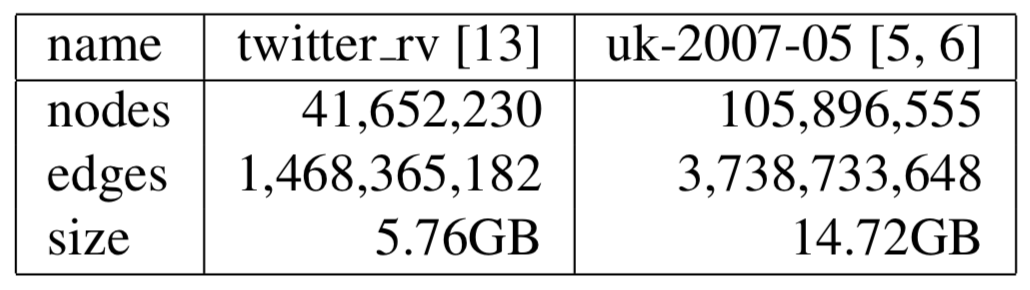
\includegraphics[width=0.65\textwidth]{dataset}
  \end{center}
  
  \vspace{0.5cm}

  \begin{center}
    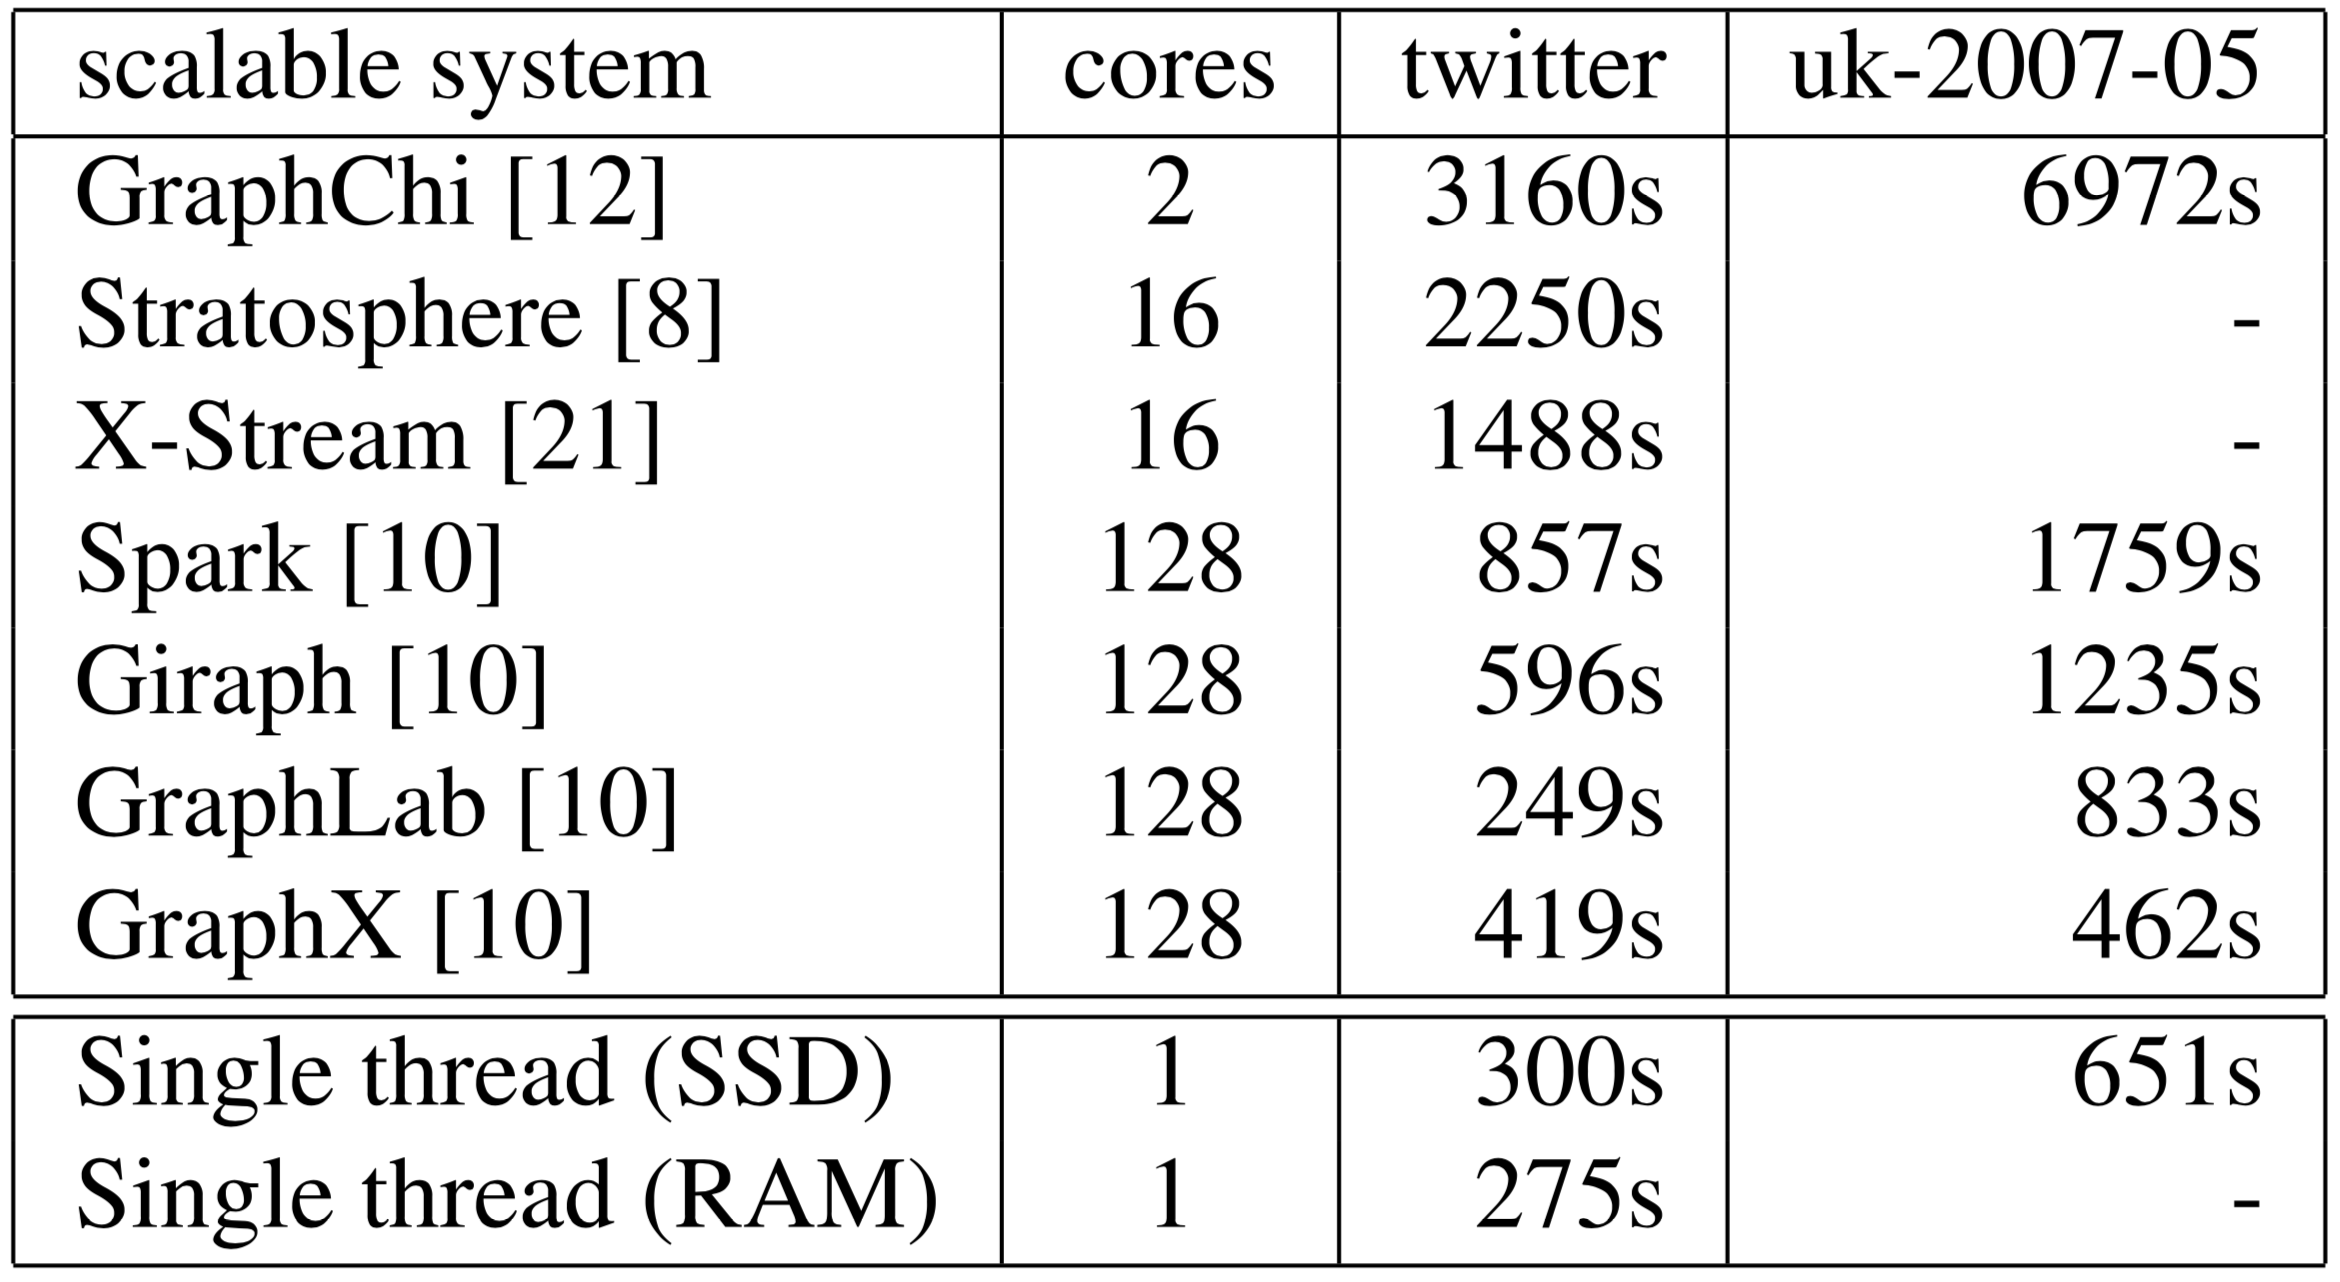
\includegraphics[width=0.75\textwidth]{pagerank}
  \end{center}
\end{frame}

\begin{frame}{Label Propagation (Connected Components)}

  \vspace{0.25cm}

  A common machine learning technique

  \vspace{0.5cm}

  \begin{center}
    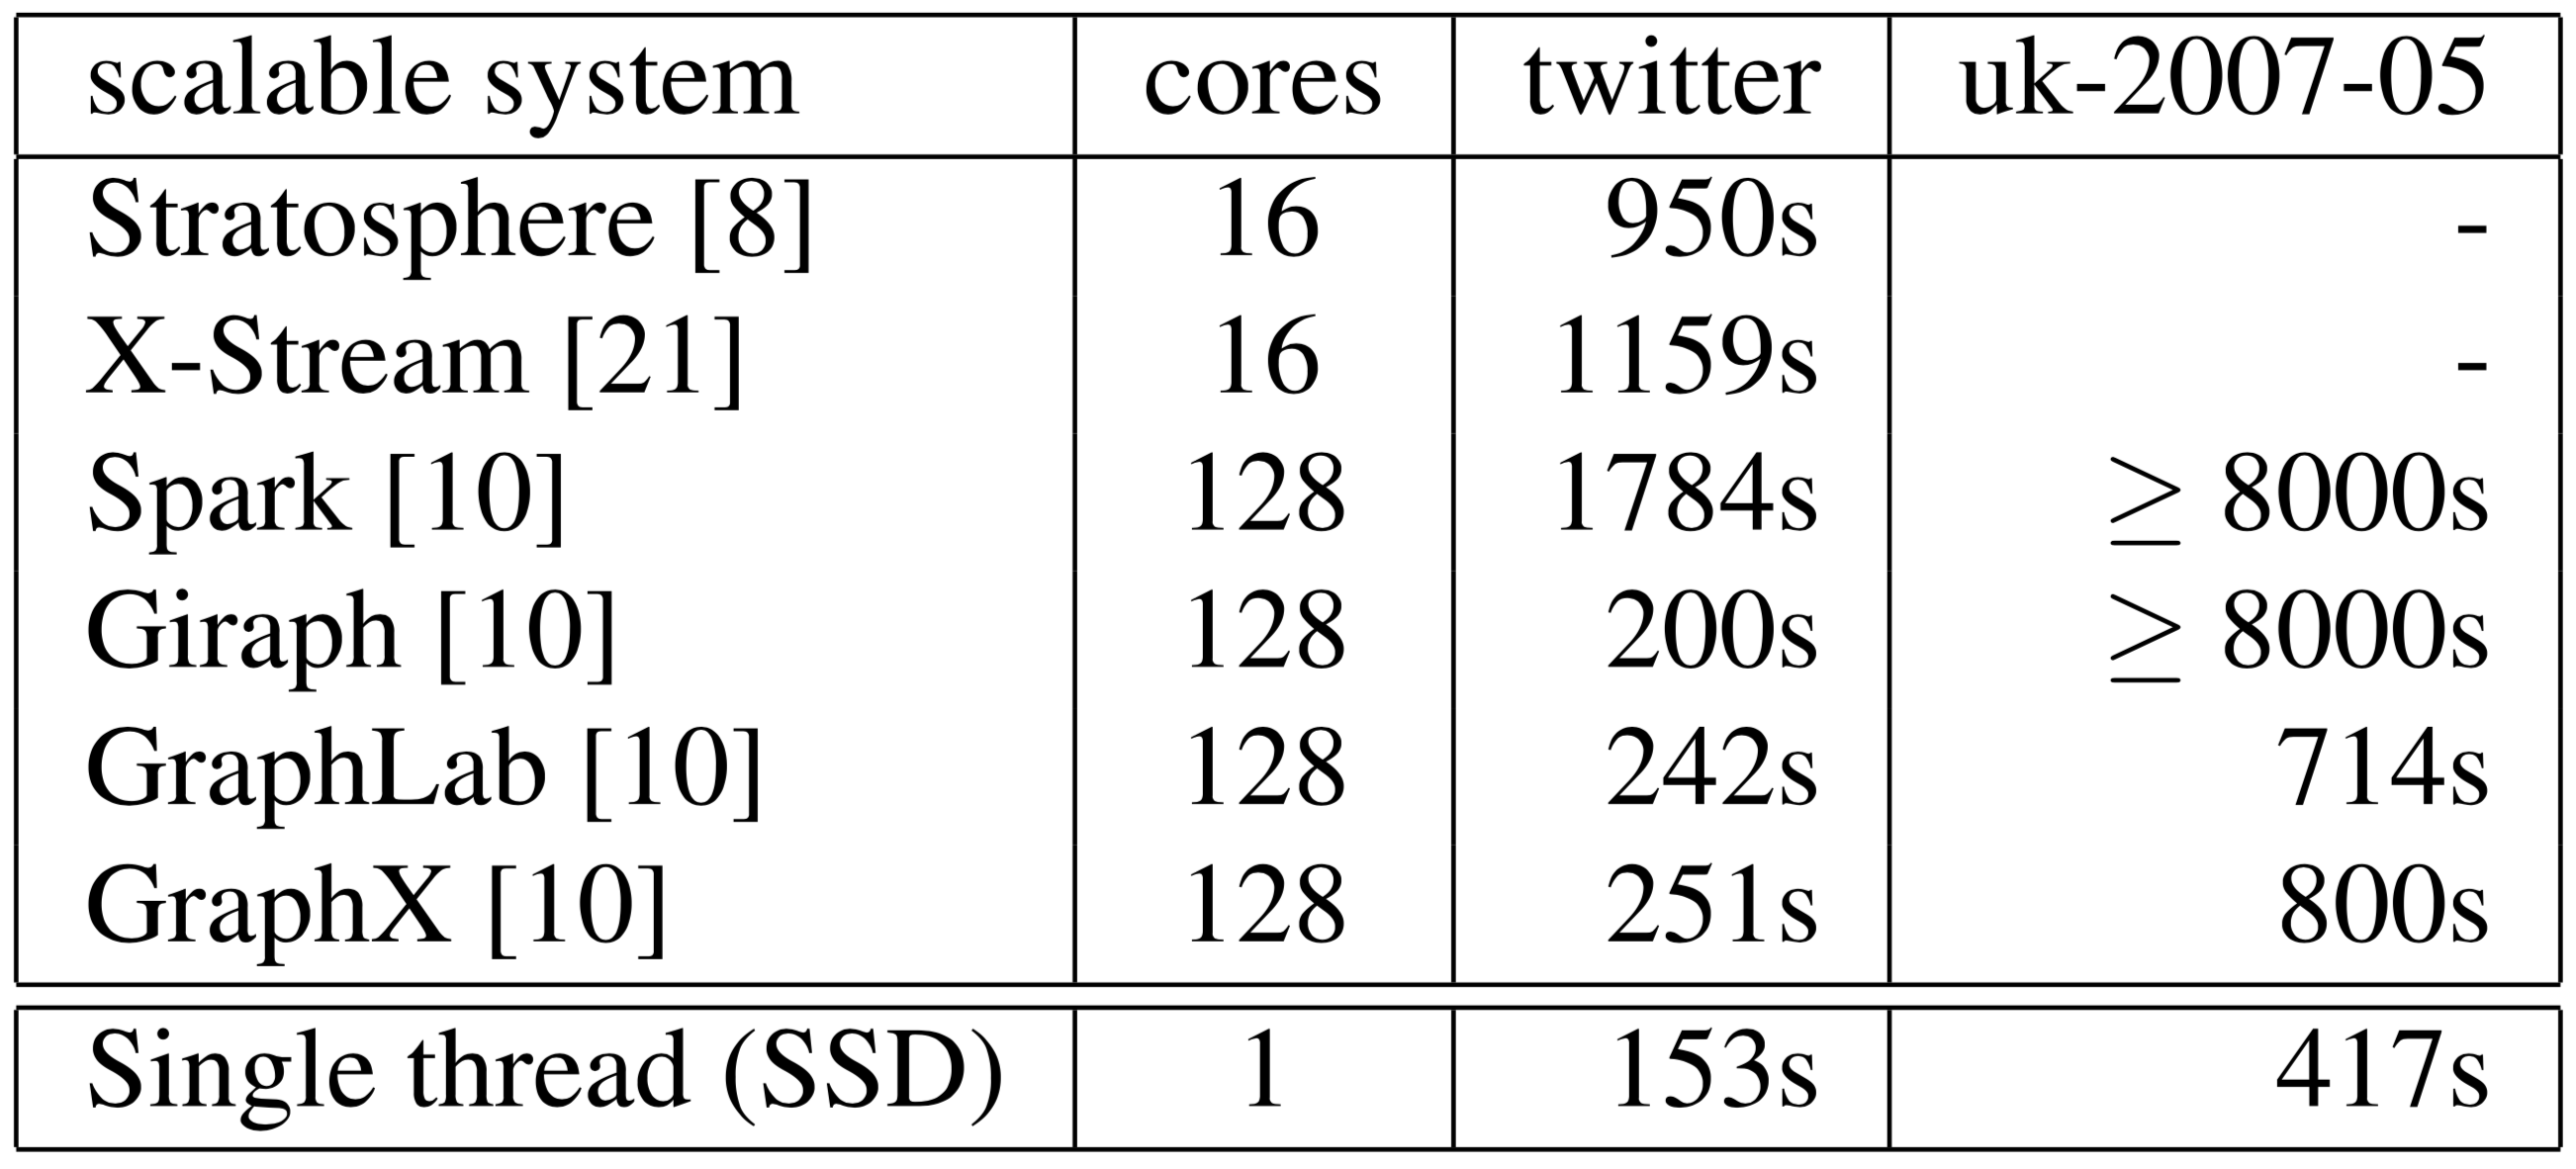
\includegraphics[width=0.75\textwidth]{label-propagation}
  \end{center}
\end{frame}